\let\negmedspace\undefined
\let\negthickspace\undefined
\documentclass[journal]{IEEEtran}
\usepackage[a5paper, margin=10mm, onecolumn]{geometry}
\usepackage{lmodern} % Ensure lmodern is loaded for pdflatex
\usepackage{tfrupee} % Include tfrupee package

\setlength{\headheight}{1cm} % Set the height of the header box
\setlength{\headsep}{0mm}     % Set the distance between the header box and the top of the text

\usepackage{gvv-book}
\usepackage{gvv}
\usepackage{cite}
\usepackage{amsmath,amssymb,amsfonts,amsthm}
\usepackage{algorithmic}
\usepackage{graphicx}
\usepackage{textcomp}
\usepackage{xcolor}
\usepackage{txfonts}
\usepackage{listings}
\usepackage{enumitem}
\usepackage{mathtools}
\usepackage{gensymb}
\usepackage{comment}
\usepackage[breaklinks=true]{hyperref}
\usepackage{tkz-euclide} 
\usepackage{listings}
\def\inputGnumericTable{}                                 
\usepackage[latin1]{inputenc}                                
\usepackage{color}                                            
\usepackage{array}                                            
\usepackage{longtable}                                       
\usepackage{calc}                                             
\usepackage{multirow}                                         
\usepackage{hhline}                                           
\usepackage{ifthen}                                           
\usepackage{lscape}

\begin{document}

\bibliographystyle{IEEEtran}
\vspace{3cm}

\title{8.ex-4}
\author{EE24BTECH11052 - Rongali Charan}
% \maketitle
% \newpage
% \bigskip
{\let\newpage\relax\maketitle}

\renewcommand{\thefigure}{\theenumi}
\renewcommand{\thetable}{\theenumi}
\setlength{\intextsep}{10pt} % Space between text and floats

\textbf{Question:}
\newline
Find the area of the region in the first quadrant enclosed by $x$-axis, line $y=x$ and the circle $x^2 + y^2 = 32$.

\textbf{Theoritical solution:}
\newline
Let the equation of the line be repsented as
\begin{align}
	\vec{x} = \vec{h} + \kappa \vec{m} \text{, where } \vec{h} = \myvec{0\\0} \text{ and } \vec{m} = \myvec{\frac{1}{\sqrt{2}} \\ \frac{1}{\sqrt{2}}}
\end{align}
Let the equation of the circle be 
\begin{align}
    \vec{x}^{\top} V \vec{x} + 2\vec{u}^{\top}\vec{x} + f = 0 \text{, where } V = \myvec{1 & 0\\0 & 1} \text{, } \vec{u} = \myvec{0\\0} \text{ and } f = - 32
\end{align}

Point of intersection of the line with the circle is given by $x_i = h + \kappa_im$, where $\kappa_i$ is calculated as,

\begin{align}
    k_i=\frac{1}{\vec{m}^\top V \vec{m}}\brak{-\vec{m}^\top \brak{Vh+\vec{u}}\pm \sqrt{\sbrak{\vec{m}^\top \brak{Vh+\vec{u}}}^2-g\brak{h}\brak{\vec{m}^\top V \vec{m}}}}
\end{align}

Substituting the values, we get,
\begin{align}
	k_i &= \pm 4\sqrt{2}\\
    x_i &= \pm \myvec{4\\4}
\end{align}
As we are only considering the first quadrant, we take the point of intersection as $\myvec{4\\4}$.
\newline
For finding the area enclosed $A$, we split the area into $2$ parts $A_1$ and $A_2$ such that
\begin{align}
    A &= A_1 + A_2 \label{eq:total_area} \\
    A_1 &= \int_{0}^{4} x \, dx \\
    &= \sbrak{\frac{x^2}{2}}_{0}^{4} \\
    &= 8 \\
    A_2 &= \int_{4}^{4\sqrt{2}} \sqrt{32 - x^2} \, dx \\
    &= \sbrak{\frac{x\sqrt{32 - x^2}}{2} + 16\sin^{-1}{\frac{x}{4\sqrt{2}}}}_{4}^{4\sqrt{2}} \\
    &= 4\pi - 8 \\
    \therefore A &= A_1 + A_2 = 4\pi \approx 12.56637
\end{align}
\textbf{Computational Solution:} Trapezoidal rule
\newline
For finding the approximate area enclosed using numerical methods, we use the Trapezoidal method. We split the area into multiple small trapeziums \brak{\text{like small strips}}, and we sum up all the trapezium areas to find the total area. 
\newline
We discretize the range of $x$-coordinates with uniform step-size $h \to 0$, such that the discretized points are $x_0$, $x_1$, $\dots$, $x_n$ and $x_{n + 1} = x_n + h$.
\newline
Let the sum of trapizoidal areas till $x_n$ be $A_n$ and $y = y\brak{x}$, then we write the $\textbf{difference equation}$,
\begin{align}
    A_n &= \frac{h}{2}\brak{y\brak{x_0} + y\brak{x_1}} + \frac{h}{2}\brak{y\brak{x_1} + y\brak{x_2}} + \dots + \frac{h}{2}\brak{y\brak{x_{n - 1}} + y\brak{x_{n}}}\\
    A_n &= h\brak{\frac{y\brak{x_0}}{2} + y\brak{x_1} + y\brak{x_2} \dots \frac{y\brak{x_n}}{2}}\\
    A_{n + 1} &= A_n + \frac{h}{2}\brak{y\brak{x_{n + 1}} + y\brak{x_n}} \text{, } x_{n + 1} = x_n + h\\
    A_{n + 1} &= A_n + \frac{h}{2}\brak{y\brak{x_n + h} + y\brak{x_n}}\\
\end{align}
By the first principle of derivative,
\begin{align}
    y^{\prime}\brak{x} &= \lim_{h\to0} \frac{y\brak{x + h} - y\brak{x}}{h}\\
    y\brak{x + h} &= y\brak{x} + h\brak{y^{\prime}\brak{x}} \text{, } h\to0
\end{align}
Rewriting the difference equation, we get,
\begin{align}
    A_{n + 1} &= A_n + \frac{h}{2}\brak{y\brak{x_n} + hy^{\prime}\brak{x_n} + y\brak{x_n}}\\
    A_{n + 1} &= A_n + h\brak{y\brak{x_n} + \frac{h}{2}y^{\prime}\brak{x_n}}\\
    A_{n + 1} &= A_n + hy\brak{x_n} + \frac{h^2}{2}y^{\prime}\brak{x_n}
\end{align}

For the given area enclosed, we take
\begin{align}
    y\brak{x} =
    \begin{cases}
        x & \quad 0 < x < 4\\
	    \sqrt{32 - x^2} & \quad 4 < x < 4\sqrt{2}
    \end{cases}
\end{align}

Substituting $y\brak{x}$, the equation becomes,
\begin{align}
    A_{n + 1} &=
    \begin{cases}
        A_n + h x_n + \frac{h^2}{2} & \quad 0 < x_n < 4\\
	    A_n + h\sqrt{32 - x_n^2} + \frac{h^2}{2}\brak{\frac{-x_n}{32 - x_n^2}} & \quad 4 < x_n < 4\sqrt{2}
    \end{cases}\\
    x_{n + 1} &= x_n + 1
\end{align}

Computational Area: 12.56576
\newline
Theoritical Area: 12.56637
\newline
Plotting the given equations, we get the following plot.

\begin{figure}[h!]
   \centering
   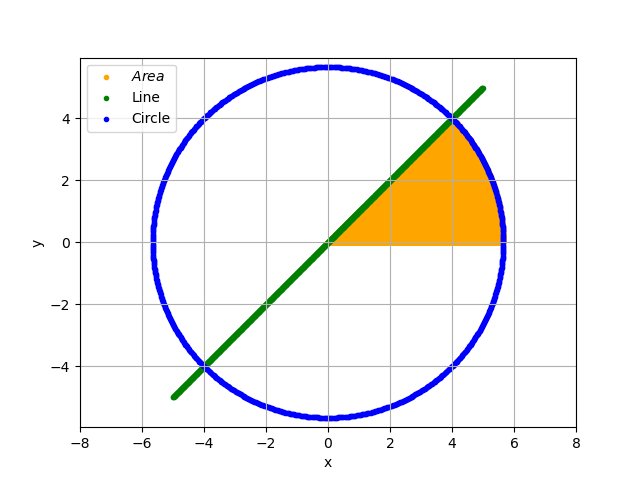
\includegraphics[width=0.7\columnwidth]{figs/graph.png}
    \caption{Shaded area with the circle and line}
   \label{label}
\end{figure}

\end{document}
